% Referencias: https://pad.riseup.net/p/OQTBcHf0BfTa

\documentclass[12pt]{article}

\usepackage[utf8]{inputenc}
\usepackage{sbc2003}
\usepackage{graphicx,url}
\usepackage[english]{babel}   
%\usepackage[latin1]{inputenc}  
\usepackage[round,sort,nonamebreak]{natbib}

\sloppy

\title{FFT benchmark on Android devices: Java versus JNI}

\author{Deusany Junior\inst{1} \and Max Rosan\inst{1} \and André
Bianchi\inst{1} \and Marcelo Queiroz\inst{1}}


\address{Computer Science Department -- University of São Paulo
         \email{\{dj,max,ajb,mqz\}@ime.usp.br}}

\graphicspath{{./img/}}


\begin{document}

\maketitle

%-----------------------------------------------------------------------------
\begin{abstract}
%-----------------------------------------------------------------------------

This work presents a comparison of running times for Java and C/C++
implementations of FFT computation on Android devices. We compare a pure Java
implementation with the widely used FFTW library that is run using the JNI,
and we also consider the possibility of multithreading. 35 different devices
were benchmarked and here we discuss results on specific combinations of
device model and operating system version. We also discuss similarities
between mono and multi threaded  versions of FFTW on multi core devices and
consider when developers can take advantages of each approach.

\end{abstract}


%-----------------------------------------------------------------------------
\section{Introduction}
%-----------------------------------------------------------------------------

With  the increasing availability of mobile devices comes the possibility of
using (relatively) low-cost, wireless hardware embedded with plenty of sensors
to perform real-time Digital Signal Processing on live artistic performances.
Some mobile applications require DSP to react on users interaction or to
process audio signals to generate effects or extract characteristics.
The Fast Fourier Transform (FFT) is an important algorithm for signal
processing applications that can be used in many of these scenarios.
%, for example, to help identifying an input signal's pitch.
% ajb: acho que pra deixar o exemplo anterior tem que colocar algum exemplo de
% não-audio também.

Considering that FFT takes $O(n\log{n})$ time (where $n$ is the FFT block
length in samples) \citep{CooleyTukey}, developers need to take care with some
FFT algorithmic characteristics during application development aiming to avoid
issues on devices with low performance. There are many different models of
mobile devices available on the market and the variety is growing everyday.

FFTW (http://www.fftw.org/) is one of the fastest and most used libraries to
calculate FFT \citep{6118781}, and its use to process signals on Android
devices consists on a step forward on real time signal processing on mobile
devices. One approach that can make it even more feasible to do real time
processing on Android devices is to use multi threading when available. The
FFTW library includes options for running mono and multithread FFTs.


Nowadays, multicore devices are becoming cheaper thus turning the
multi-threaded approach into a good choice for developers. On the other hand,
as Android devices also need to take care of saving battery as a primordial
action, using more than one processor for just the FFT task is not an easy
practice. Another important consideration concerns devices' specific operating
system implementations that might split the processing into two or more cores
or not. Testing multi threaded methods can have strange results depending on
device models' peculiarities (http://bigflake.com/systrace/).

This work presents the latests results of a benchmark  testing real-time FFT
task of varying sizes using a Java implementation and FFTW library, which is
written using C/C++ code, running on top of the JNI.
% TODO: add ref for JNI
We collected results from 35 different devices and obtained statistics of some
specific combinations of  device model and operating system version. We
discuss similarities and differences between mono thread and multi threaded
versions of FFTW on multi core devices and consider when developers can  take
advantages of each approach.

%-----------------------------------------------------------------------------
\section{Related work}
%-----------------------------------------------------------------------------

Although audio processing is API dependent in earlier devices, the Android
Gingerbread version (2.3)added OpenSL native audio library into the system
\citep{Pathak2011,LazzaLAC}. Evolution of mobile processors also had large
influence on audio application development. 
% TODO: o parágrafo acima pode ser melhor contextualizada para o trabalho
% atual?

Since JNI is also supported on Android devices, it is possible to use all the
JNI 1.6 features on Android, with exception of some features described in
\cite{MakingMusicalApps}.  Recent  efforts have been mixing the Android
platform with traditional real-time DSP software, such as Csound
\citep{LazzaLAC} and Pure  Data \citep{MakingMusicalApps}. Both of these
approaches make use of the JNI (https://developer.android.com/tools/sdk/ndk/)
to mix C/C++ code with Java code to wrap libraries and allow these
environments to run on the Android OS.  Our approach, on the other hand, uses
pure Java code to implement a minimal GUI and real-time DSP model, and native
code to carry performance measurements and compare Java and C/C++ FFT
implementations.



%-----------------------------------------------------------------------------
\section{Methodology}
%-----------------------------------------------------------------------------

To  get a feel of what it is like to use Android devices for real-time DSP, we
have set up an environment to run arbitrary algorithms over an audio stream
divided into blocks of N samples, allowing for the variation of algorithm
parameter during execution. The software used is the Android DSP benchmarking application
developed by \cite{ajbmqzSMC2012}, with some modifications to test
the methods selected on this work and open source code available at
https://github.com/andrejb/DspBenchmarking/.


To compare the performance of different implementations of the FFT algorithm
on Android devices, we devised three processing scenarios of a one-way FFT: using a pre Java implementation, using FFTW mono threaded and using FFTW multi threaded.
As the FFTW  implementation is coded using C (or C++?), JNI was used to include the
code into the benchmark tests. In each scenario, the program keeps track  of
the full DSP callback period (including conversion between PCM and  floating
point sample representation, timekeeping code and sample enqueueing for playback),
and also the actual DSP algorithm execution time. The  main purpose of using
these methods is to confirm the advantages of  using the FFTW against normal
FFT, and figure out the relevance of using  FFTW multi-thread for different
block sizes.

All  performance measurements are made by the application started by the
user. User interactive assistance is kept at a bare minimum, by starting  the
experiment and pressing a button to e-mail the results to the  authors. To
obtain as many results as possible, we decided to launch a  call for
participation on the internet, making a total of 35 different  devices.
Instructions were sent to stop all applications and turn off communication
(tests could only be started after the user enabled flight mode) to impose an
"idle" scenario on every device. The result of imposing these  constraints is
an overall experiment that automatically cycles through all benchmarking
algorithms, and then sends an e-mail report with results back to the authors.



%-----------------------------------------------------------------------------
\section{Results and discussion}
%-----------------------------------------------------------------------------



\begin{figure}[h!]
\begin{center}
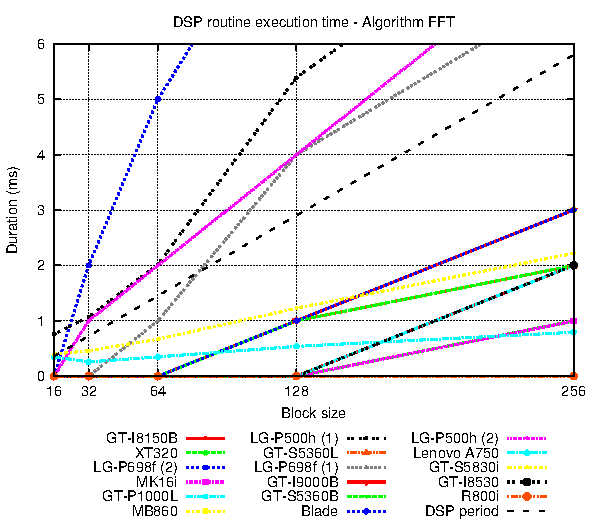
\includegraphics[width=0.7\textwidth]{img/FFT_ALGORITHM-2-a.pdf}
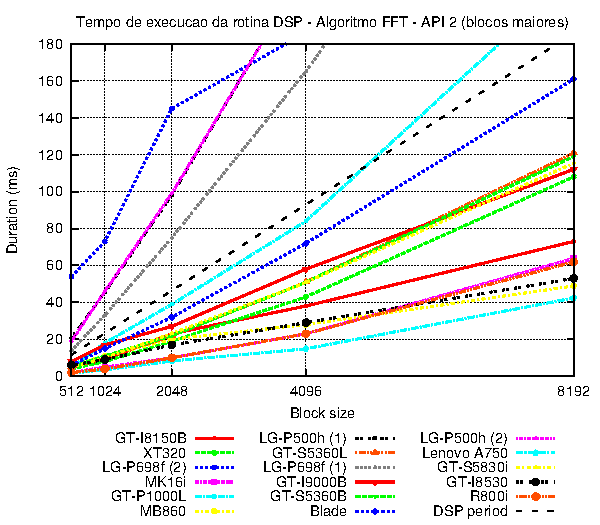
\includegraphics[width=0.7\textwidth]{img/FFT_ALGORITHM-2-b.pdf}
\end{center}
\caption{Benchmark of FFT implemented in pure JAVA in devices with API version
2.X for smaller (above) and larger (below) block sizes.}
\label{fig:alg-fft}
\end{figure}

\begin{figure}[h!]
\begin{center}
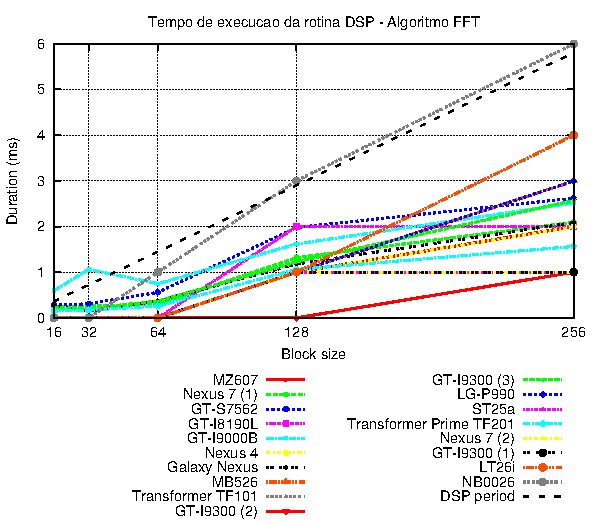
\includegraphics[width=0.7\textwidth]{img/FFT_ALGORITHM-4-a.pdf}
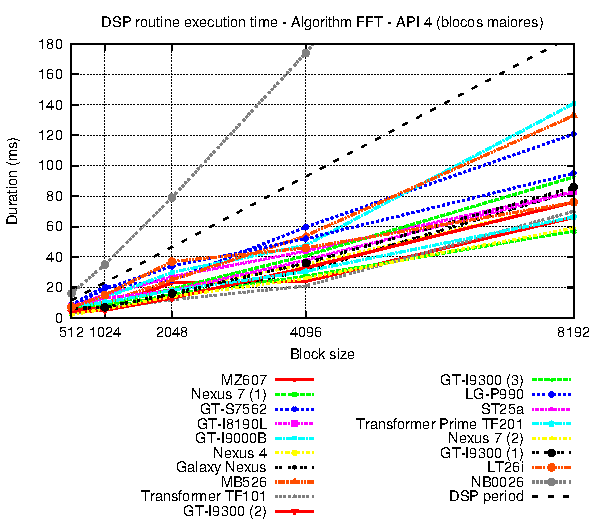
\includegraphics[width=0.7\textwidth]{img/FFT_ALGORITHM-4-b.pdf}
\end{center}
\caption{Benchmark of FFT implemented in pure JAVA in devices with API version
4.X for smaller (above) and larger (below) block sizes.}
\label{fig:alg-fft}
\end{figure}

\begin{figure}[h!]
\begin{center}
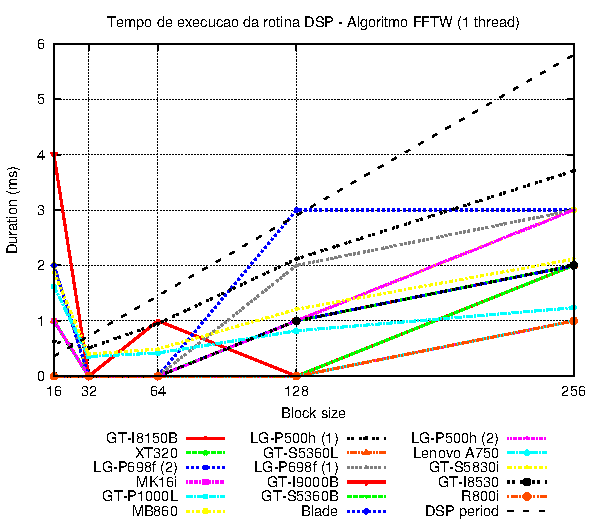
\includegraphics[width=0.7\textwidth]{img/FFTW_MONO-2-a.pdf}
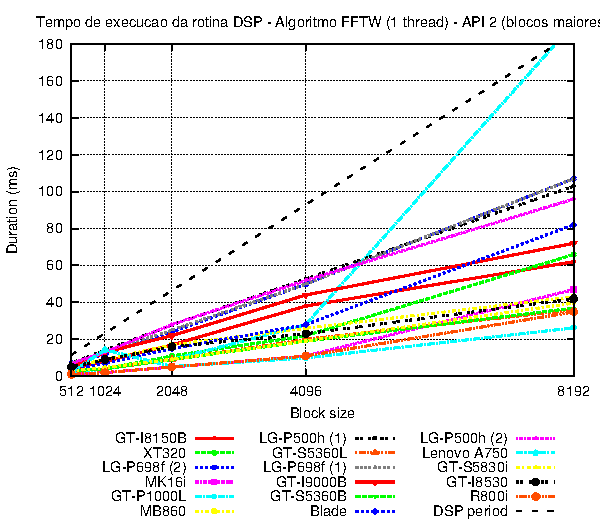
\includegraphics[width=0.7\textwidth]{img/FFTW_MONO-2-b.pdf}
\end{center}
\caption{Benchmark of FFT using monothread FFTW library in native code in
devices with API version 2.X smaller (above) and larger (below) block sizes.}
\label{fig:alg-fftw-mono}
\end{figure}

\begin{figure}[h!]
\begin{center}
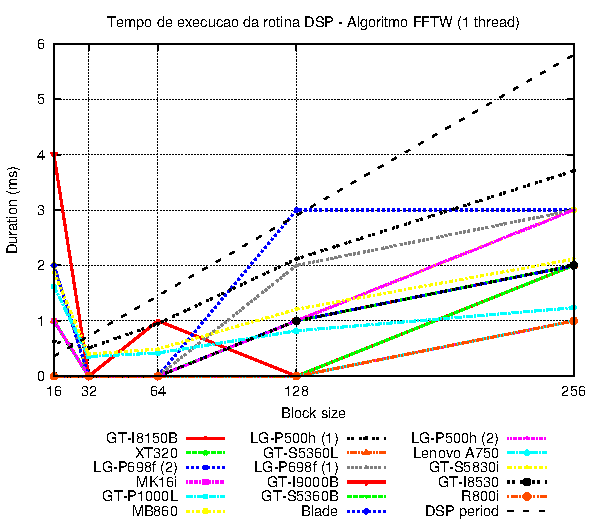
\includegraphics[width=0.7\textwidth]{img/FFTW_MONO-2-a.pdf}
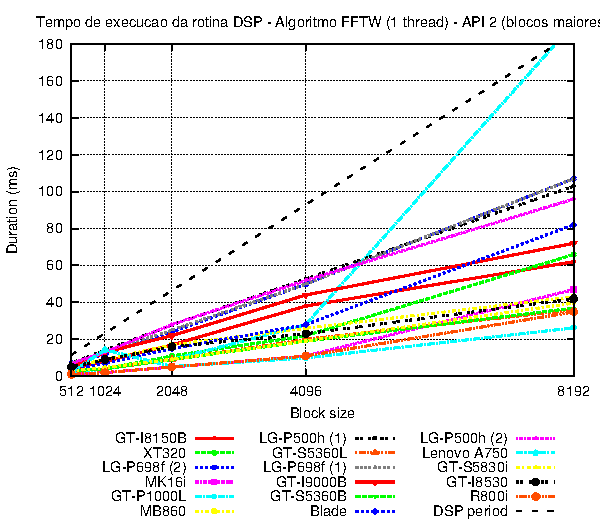
\includegraphics[width=0.7\textwidth]{img/FFTW_MONO-2-b.pdf}
\end{center}
\caption{Benchmark of FFT using monothread FFTW library in native code in
devices with API version 4.X smaller (above) and larger (below) block sizes.}
\label{fig:alg-fftw-mono}
\end{figure}

\begin{figure}[h!]
\begin{center}
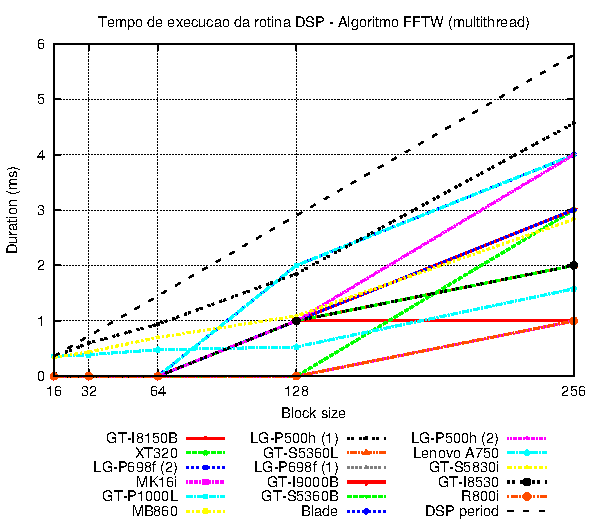
\includegraphics[width=0.7\textwidth]{img/FFTW_MULTI-2-a.pdf}
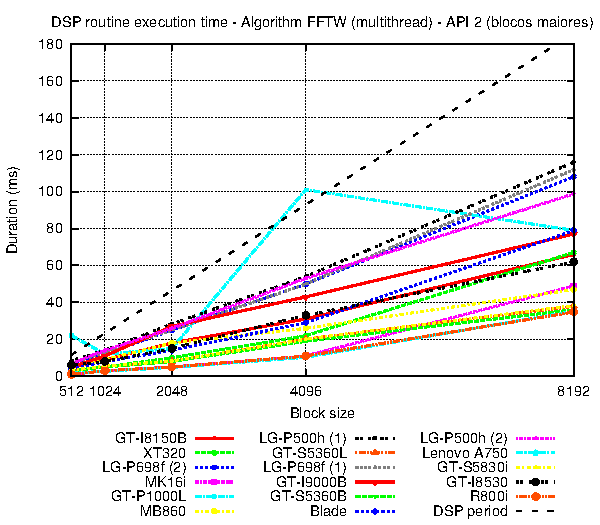
\includegraphics[width=0.7\textwidth]{img/FFTW_MULTI-2-b.pdf}
\end{center}
\caption{Benchmark of FFT using multithread FFTW library in native code in
devices with API version 2.X for smaller (above) larger (below) block sizes.}
\label{fig:alg-fftw-multi}
\end{figure}

\begin{figure}[h!]
\begin{center}
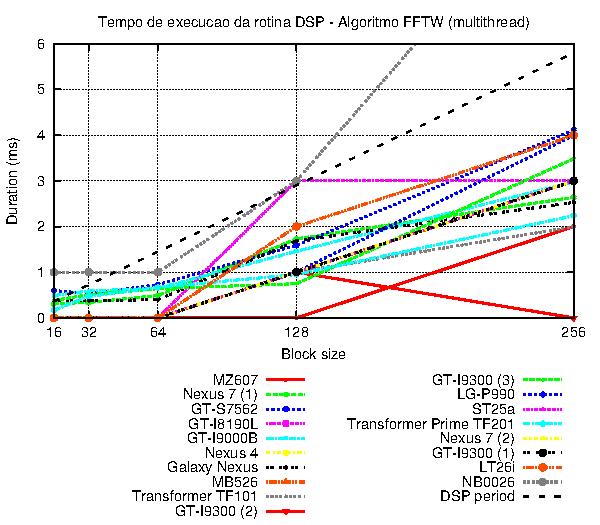
\includegraphics[width=0.7\textwidth]{img/FFTW_MULTI-4-a.pdf}
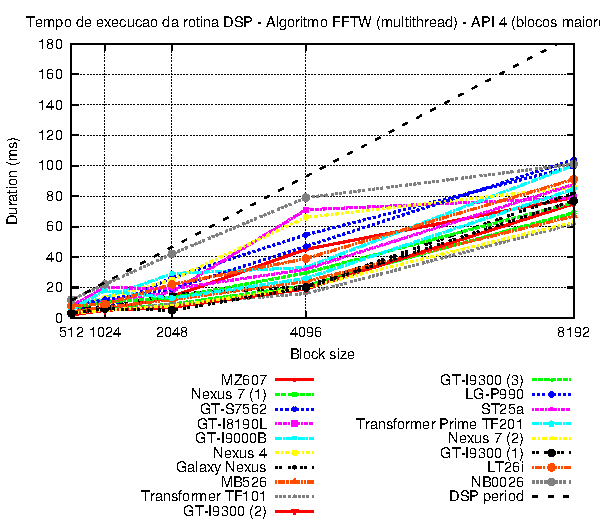
\includegraphics[width=0.7\textwidth]{img/FFTW_MULTI-4-b.pdf}
\end{center}
\caption{Benchmark of FFT using multithread FFTW library in native code in
devices with API version 4.X for smaller (above) larger (below) block sizes.}
\label{fig:alg-fftw-multi}
\end{figure}


Figures \ref{fig:alg-fft}, \ref{fig:alg-fftw-mono} and
\ref{fig:alg-fftw-multi} show the time taken by each of the FFT algorithms to
be executed for different block sizes and device models. By comparing the FFT
and FFTW monothread results, on Figures \ref{fig:alg-fft} and
\ref{fig:alg-fftw-mono} respectively, it's possible to notice that FFTW
monothread is faster than FFT when blocks larger than 16 samples are
considered. Because of the overhead caused by the loading of a dynamic
library, the results of FFTW monothread for blocks with size equal to 16 are
worse than the FFT ones. As the FFTW library is loaded when the algorithm is
executed for the blocks larger than 16, the overhead due to the initialization
of the library is not noticed for larger blocks. The same happens to FFTW
multithread: it is executed after FFTW monothread and therefore there is no
overhead for the initialization of the library.


It's also possible to notice that FFTW has worse performance when it is used
with multiple threads. It so happens that kernel of Android shifts threads
of a program to different cores provided that they are CPU-intensive and has
been running for a sustained period. Threads created by FFTW are
CPU-intensive, however the tested block sizes are not large enough to cause the
threads to be shifted to different cores. In \cite{systrace}
there are some experiments using systrace
\cite{systraceandroid} that point out
what happens to CPU-intensive threads on Android multicore devices. Some
Android devices, like Sony Xperia U \cite{xperiauspecs}, have all the cores enabled all the time,
but others, like Motorola Xoom2 [ref], enable additional cores according to the conditions
explained before. This behaviour occurs because turning one core on
is an expensive process in terms of energy consumption, so Android tries to keep  some cores
disabled until there is an application CPU-intensive need them for a considerable
time interval \cite{systrace}. Also, this behaviour can be altered by manufacturers when shipping distinct device models and so there is no default behaviour that can be expected in general.

% ajb: verificar se a última frase do parágrafo anterior, que adicionei, é verdadeira.


[ref] 


\subsection{ Conclusion and future work}

FFT is an algorithm widely used in signal processing applications. Applications like speech recognition
and audio processing can be found on mobile devices like Android ones. Considering how powerful the CPU
in those devices are becoming nowadays, executing FFT on them can be a better option than transfering data
blocks to a server side, which is a common option made by applications. It was showed here that it is possible to use FFT even in applications with
real-time processing requirements. Besides, the performances of FFT implemented in pure Java and
FFTW executing on the JNI were compared.

The FFT implemented in pure Java had a worse perfomance than the implementation using FFTW through JNI. This shows that using FFTW with JNI can be a better option than using FFT implemented using pure Java. On other hand it is expensive to load a dynamic library for using JNI, so FFTW spent much more time than plain Java FFT to compute the first block, even though opposite occurred for larger blocks sizes.

The option of using FFTW for doing computing the FFT in parallel by using threads was also considered. It was expected that doing calculations in parallel would reduce the time needed to compute the FFT. FFTW uses threads to implement calculations in parallel. Threads are expensive and unnecessary in devices with only one core, so on devices that contain only one core FFTW multithread had a worse performance than FFTW monothread. However, depending on device model, Android has scheduling politics that shift threads to different cores only if it has been running for considerable time and it is CPU-intensive. Due to those politics and the size of the blocks, that FFTW multithread had a worse performance even on devices where there are more than one CPU core. So it is interesting to use FFTW with multiple threads when that those threads keep running for a long enough time. 

% conclusion

 Considering the limitation of resources of a mobile device, like CPU and memory,
 it is necessary to be careful with the extra overhead incurred by native
code called through JNI. However, there are a lot of libraries  and
applications written in languages like C and C++ that can be  compiled to
native code and run on processors used by most of the Android
devices, like ARM and Intel chips.

By using
JNI, developers can have the advantages of including FFTW on their application
instead of reimplementing the algorithm in Java, while achieving
better performance than code implemented in pure Java. 


The  use of native code does not automatically imply better performance
because it increases application complexity and also has a cost associated
with calls to non-Java code. There are works that aim to find  performance
differences between Java and native code on different  scenarios, and conclude
that native code is indeed worse for some  applications \citep{6118781}.
Nevertheless, an implementation and
comparison with native code for real-time signal processing is needed and here we propose some results
from first experiments using JNI to test FFT on native code.

Processor  and memory consumption during an FFT transform computation depend on
the  block size and the processing method. Devices with 1GHz processors and
512 MB RAM memory are becoming cheaper and allow real time
computation of FFT on common Android devices even though Android APIs  still
have some limitations. The APIs limitations related to Linux low level
processing support are still being tested and new features have been being added on
each new Android release. The latest devices evolution are related  to multi-thread
support concerning the multi-core mobile processors era, and because of this real-time
processing is getting more attention from developer's  eyes.

Real time processing is possible depending on the amount of work being carried by the operating system in the
background. From a programming language perspective, low level code is prefered
to achieve higher performance processing whether or not the
multi-threading concept is on focus. Taking advantage of low level code is
possible using JNI (Java Native Interface) on Android applications. Even
though the main supported language is Java, JNI allows Java code to use code and
libraries written in another language like C,  C++, assembly, and others. Also, the
use of JNI also allows Java code to be embedded in  applications not written in
Java. It is supposed to be used, for example, in situations where Java applications need
to use libraries that are not implemented in Java and which code is not available or  can not be ported to Java because of low-level issues.
As Java  applications are executed on top of Java virtual machines that run on different platforms,there exists the possibility that native code may be executed faster than Java code. Thus, JNI can be  used to implement portions of critical-time code.

% ajb: no parágrafo de cima diz que JNI permite uso de assembly, e no de baixo diz que não é possível portar FFTW porque usa assembly.
% FFTW is optimized by making use of assembly code and can not be completely ported to Java due to that.


\begin{itemize}


    \item FFT perdeu para FFTW [x]


    \item FFTW teve problemas para inicialização mas conseguiu superar a FFT
    nos outros casos independente disso [x]
    http://gcc.gnu.org/ml/gcc/2004-06/msg01956.html


    \item Limitações de dispositivos devem ser consideradas [x]
    http://developer.android.com/training/articles/perf-jni.html\#unsupported


    \item FFTW  multithread não superou FFTW mono thread por não requisitar
    muito do  processador e assim o processador não atribui os processos a
    núcleos  diferentes [x]


    \item Só há vantagem em uso de multithread se o trabalho for muito grande [x]


    \item We  are preparing new tests including FFT to get a better overview
    of other  methods and libraries. Here are the next steps proposed: \# Pure
    Java multithread implementation


    \item FFT from Pure Data using libpd
    (http://puredata.info/downloads/libpd/)  that is a port of Pure Data's
    core engine which make possible to run  Pd patches as C native code over
    Android's Dalvik Java VM. 


    \item FFT from CSound on Android
    \url{http://www.csounds.com/journal/issue17/android\_csd\_player.html}


    \item FFT from supercolider on Android


    \item Testing these methods we will know the state of art on FFT
    implementation for Android devices considering the real time processing
    and also bearing in mind that the fast we compute FFT, the less battery
    draining we will have.

\end{itemize}


%\section{Acknowledgements}
%We would like to thank the members of the Computer Music Group
%(http://compmus.ime.usp.br/en/)  of the Computer Science Department of the
%Institute of Mathematics and  Statistics of the University of São Paulo. This
%work has been supported  by the funding agencies CAPES and FAPESP (grant
%2008/08632-8).


%-----------------------------------------------------------------------------
\section{References}
%-----------------------------------------------------------------------------

\bibliographystyle{apalike}

\bibliography{references}

\end{document}

